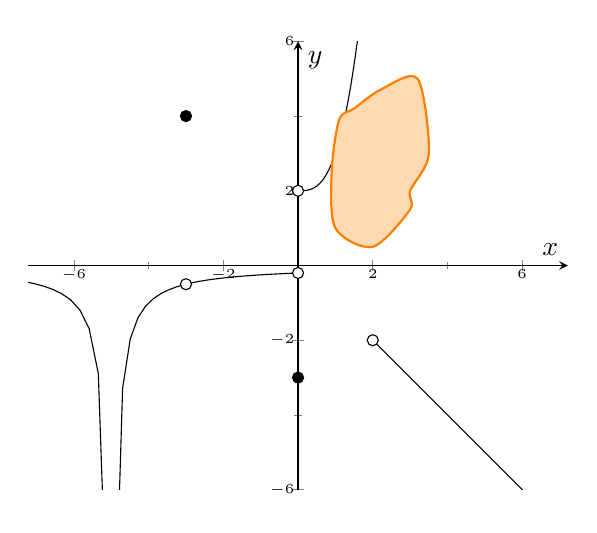
\begin{tikzpicture}
\pgfplotsset{my style/.append style={axis x line=middle, axis y line=
middle, xlabel={$x$}, ylabel={$y$}, axis equal },every tick label/.append style={font=\tiny},
yticklabel style = {font=\tiny,xshift=0.5ex},
xticklabel style = {font=\tiny,yshift=0.5ex}
}
\begin{axis}[my style, xtick={-6,-2,...,6}, ytick={-6,-2,...,6},
xmin=-3, xmax=3, ymin=-6, ymax=6,  minor tick num=1]
\addplot[domain=-11:-5.1] {1/(x+5)};
\addplot[domain=-4.9:0] {-1/(x+5)};
\addplot[domain=0:2] {x^3+2};
\addplot[domain=2:10] {abs(x-7)-7};
\addplot[mark=*,only marks] coordinates {(-3,4)(0,-3)(2,10)};
\addplot[mark=*,fill=white,only marks] coordinates {(-3,-.5)
(0,-.2)(0,2)(2,-2)};
\addplot[mark=none, orange, smooth cycle, thick, fill=orange!30] coordinates {%
   (1,1) (2,0.5) (3,1.5) (3,2) (3.5,3) (3.2, 5) (2.2, 4.7) 
   (1.5, 4.2) (1.1, 3.9) (0.9, 2.5) };
\end{axis}
\end{tikzpicture}